\chapter{Project Plan}
\section{Risk Management Procedure}
Certain risks will be faced throughout the project, though proper avoidance and mitigation plans will allow project objectives to be completed on time.
Risks will be obsessed using AHP and pairwise comparisons.
If possible, quantitative measurements, in terms of financial or class grade loss if the risk is realized, will allow comparison to determine which risks should be focused on to ensure that they are not realized.

\subsection{Risk Identification}
From previous experience, the major risks that will occur in the project will likely be related to increasing scope, unfeasible designs, insufficient resources, delayed shipments, and lack of motivation.

\subsection{Risk Avoidance}
\begin{itemize} \parskip2pt
	\item To avoid increasing scope late in the project, there will be a change moratorium to the project’s scope at the end of the senior thesis proposal class. Any additional substantial features must be put on hold until the end of the semester if time permits; all other requirements must first be completed.
	\item To avoid issues from a design becoming unfeasible, viable alternative designs will be created in the planning phase.
	\item To avoid running short of resources, proper resource management and thorough time and money planning will ensure that all resource expenditure is within budget.
	\item To avoid being affected by delayed shipments, parts will be ordered as soon as they are confirmed to be required.
	\item To avoid slipping motivation, the team will be kept in contact to create an atmosphere of team cooperation and ensure that all team members feel useful in the project.
\end{itemize}	

\subsection{Risk Mitigation}
\begin{itemize}
	\item In the case of required increased project scope, the team will collaborate and decide the new priority of tasks using AHP. The tasks will be worked in the order decided, and the team will understand which items may not be completed in time.
	\item In case a design becomes unfeasible, one of the alternate designs created in the planning phase will be pursued.
	\item In case of insufficient financial resources, the investors will be contacted, or more investors will be located to sponsor the project.
	\item If shipments are delayed, alternative distributors will be researched and ordered from to obtain the part in time.
	\item If there is a lack of motivation on the team, team outings will be planned that do not involve the project, but will allow team bonding and any personal issues to be discussed.
\end{itemize}

\section{Change Management Procedure}
Any major changes to the design will be decided with a meeting that includes all the effected developers.
Once a change has been decided on, the Resource Manager will complete the paperwork for an \gls{ecr}.
This will be submitted to Professor Detolff for review.
If the change is approved, an \gls{eco} will be used to direct the change.

\section{Work Breakdown Structure}
\begin{longtable}{|c|m{4cm}|m{4cm}|>{\centering}m{1.6cm}|m{3.5cm}|}
	\caption{Work Breakdown Structure}
	\label{table:primary} \\
	\hline \textbf{ID} & \textbf{Activity} & \textbf{Deliverable} & \textbf{Duration (Days)} & \textbf{Resources} \\ \hline
	\endfirsthead
	\multicolumn{5}{c}{\tablename\ \thetable\ -- \textit{Continued from previous page}} \\ \hline
	\textbf{ID} & \textbf{Activity} & \textbf{Deliverable} & \textbf{Duration (Days)} & \textbf{Resources} \\ \hline
	\endhead 
	\multicolumn{5}{r}{\textit{Continued on next page}} \\
	\endfoot \hline
	\endlastfoot

	\hline 1 & \multicolumn{4}{c|}{Electrical Components} \\ \hline
	1.1 & Construct test board & LED testing breakout & 7 & Components\newline Perfboard \\ \hline
	1.2 & \multicolumn{4}{l|}{Motor Driver Prototype} \\ \hline
	1.2.1 & Design motor driver PCB & Shield PCB & 30 & Eagle\newline \gls{cnc}\newline Components \\ \hline
	1.2.2 & Order motor drivers & Motor drivers & 1 & Computer \\ \hline
	1.2.3 & Construct sensor circuitry & Sensor circuitry & 14 & Eagle\newline \gls{cnc}\newline Components \\ \hline
	1.2.4 & Construct power supply & Power & 7 & Eagle\newline \gls{cnc}\newline Components \\ \hline
	1.3 & Send final motor driver PCB design to boardhouse & Final motor driver & 14 & Eagle\newline \gls{cnc}\newline Components \\ \hline
	1.4 & Construct work head controller & Work head controller & 17 & Eagle\newline \gls{cnc}\newline Components \\ \hline
	\hline 2 & \multicolumn{4}{c|}{Control Software} \\ \hline
	2.1 & \multicolumn{4}{l|}{LED Control Software} \\ \hline
	2.1.1 & Research \gls{pi} \gls{gpio} & Pi \gls{gpio} knowledge & 4 & Computer \\ \hline
	2.1.2 & Program for \gls{pi} \gls{gpio} & LED controller & 3 & Computer \\ \hline
	2.2 & \multicolumn{4}{l|}{Motor Control Software} \\ \hline
	2.2.1 & \gls{gpio} Timing research & \gls{gpio} timing understanding & 5 & Computer \\ \hline
	2.2.2 & Program motor controller & Motor controller software & 10 & Computer \\ \hline
	2.3 & \multicolumn{4}{l|}{Kinematics Control Software} \\ \hline
	2.3.1 & Research kinematics requirements & Kinematics equations & 5 & Computer\newline Calculator \\ \hline
	2.3.2 & Program kinematics equations & Kinematics software & 10 & Computer \\ \hline
	2.4 & \multicolumn{4}{l|}{G-code Interpreter} \\ \hline
	2.4.1 & G-code research & G-code understanding & 7 & Computer \\ \hline
	2.4.2 & Program G-code interpreter & G-code Software & 14 & Computer \\ \hline
	2.5 & Experiment to improve accuracy & Improved precision & 14 & Computer \\ \hline
	\hline 3 & \multicolumn{4}{c|}{Interface Software} \\ \hline
	3.1 & Interface \gls{pi} with Ethernet & Wired TCP/IP Interface & 10 & Computer \\ \hline
	3.2 & Interface \gls{pi} with WiFi & Wireless TCP/IP Interface & 15 & Computer \\ \hline
	3.3 & Program ability to upload G-code & TCP/IP G-code Upload & 10 & Computer \\ \hline
	3.4 & Program website for monitoring & HTTP Website & 21 & Computer \\ \hline
	\hline 4 & \multicolumn{4}{c|}{System Testing} \\ \hline
	4.1 &Verifying motor frequency accuracy&The stepper motors will have a minimum pulse frequency of 10kHz and a margin of pulse frequency error of  $\pm $5\% & 7 & Computer \newline Oscilloscope \\ \hline
	4.2 &Verifying communication channels &  G-Code will be transfered through TCP/IP. & 7 & Computer \\ \hline
	4.3 &Verifying power ratings& The system will work with any power supply that can output 14 to 36V and up to 10A. & 7 & Oscilloscope \newline Multimeter \newline Power resistors \\ \hline
	4.4 &Verifying control capabilities&  The system will be able to drive 4 stepper motors, 1 DC motor, 16 GPIO pins, 1 Emergency Stop and 4 Home switches. & 7 & Computer \newline Motors \newline LEDs\\ \hline
	4.5 & Verifying safety shutdown&The CPU will not exceed 60$^\circ$ Celsius. & 7 & Test oven\\ \hline
	\hline 5 & \multicolumn{4}{c|}{Integration Testing} \\ \hline
	5.1 & Test web interface & Web interface & 7 & Computer\\ \hline
	5.2 & Test master controller & Master controller & 7 & Computer \newline Oscilloscope \newline Power supply \\ \hline
	5.3 & Test motor controller & Motor controller & 7 & Oscilloscope \newline Power supply\\ \hline
	5.4 & Test motor driver board & Motor driver board& 7 & Oscilloscope \newline Power supply\\ \hline
	\hline 6 & \multicolumn{4}{c|}{Unit Testing} \\ \hline
	6.1 & Test G-code interpreter& G-code interpretation& 7 & Computer\\ \hline
	6.2 & Test stepper pulse timing & Stepper pulse timing& 7 & Computer \newline Oscilloscope\\ \hline
	6.3 & Test user command interpretations & User command interpretation& 7 & Computer\\ \hline
	\hline 7 & \multicolumn{4}{c|}{Product Management} \\ \hline
	7.1 &Documenting work&Update Log Books & On-going & Log book\newline Writing utensil \\ \hline
	7.2 &Keeping project management charts up to date&Update project management charts & On-going & Computer\\ \hline
	7.3 &Emergency backups&Back up documentation & On-going & Computer\\ \hline
	7.4 &Communicating&Team meetings & On-going & Log book \newline Communication device\\ \hline
	7.5 &Keeping in budget&Budget reviews & On-going & Budget \newline Record book\\ \hline
	7.6 &Keeping on time&Project progress reviews& On-going & Gantt chart\\ \hline
	7.7 &Communicating progress &Meetings with professors& On-going & Computer \newline Log book\\ \hline
\end{longtable}
\subsection{Project Specific Deliverables}
There are 5 Project Specific Deliverables.
	\begin{enumerate}
		\item  The stepper motors will have a minimum pulse frequency of 10kHz and a margin of pulse frequency error of  $\pm $5\%.
		\item G-Code will be transfered through TCP/IP.
Software will be developed using IEEE Std 830-1998 Recommended Practice for Software Requirements Specifications.
		\item The system will work with any power supply that can output 14 to 36V and less than 10A.
		\item The system will be able to drive 4 stepper motors, 1 DC motor, 16 GPIO pins, 1 Emergency Stop and 4 Home switches.
		\item The CPU will not exceed 60$^\circ$ Celsius. 
	\end{enumerate}
\subsection{Design Review}
The initial project review raised the concern that the scope was too large and not well defined.
This led to a reevaluation of the project from a full mechanical system to a driver board.
This helped make the project more concrete in direction and functionality while still being difficult enough for four engineers.

Design Reviews will happen continually throughout the project development. 
Specific review sessions will happen as major problems arise but will happen at least once a week at weekly team meetings.
\subsection{Risk Management Review}
Risks were presented in a project review session with Professor Detloff.
The project seemed not feasible in amount of development time allowed.
This was reviewed and the alternate of the \gls{cnc} Interface was selected to reduce the project scope to a manageable size. 
All other risk avoidance and mitigation techniques are still being used.   

Risk management reviews will happen before any major decision on the project.
The whole team will be present for these reviews. 
This will lower the chance that any risk will be over looked.

\subsection{Stakeholder, Communication, and Resource Review}
\begin{figure}[H]
\centering
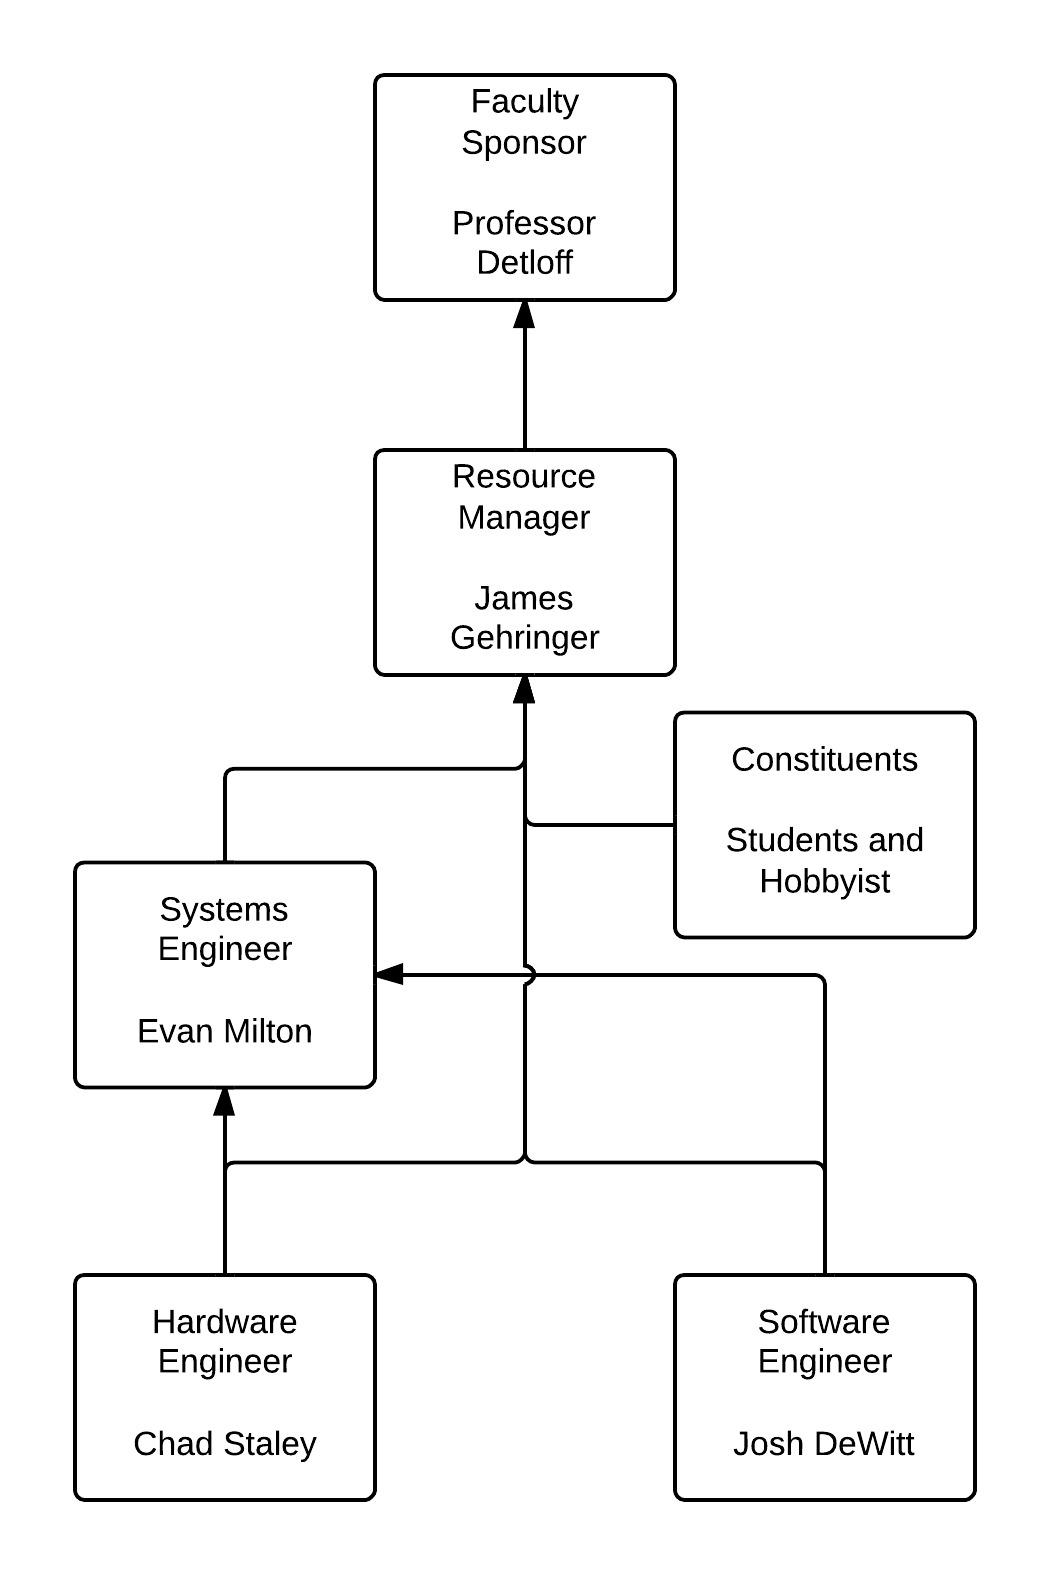
\includegraphics[width=0.6\textwidth]{shc.jpeg}
\caption{Stakeholder Chart}
\label{fig:Stakeholder Chart}
\end{figure}
The Stake Holder chart has been reviewed and updated to the Figure 7.1.
These are all the parties that are currently invested in the project. 
If more parties become invested, then the organization and chart will be revisited. 

Communication techniques being used are successful in keeping all involved informed.
As the project progresses, more face-to-face team meetings will occur.
In the event that communication channels start to break down, a team meeting will be called and new processes will be evaluated. 

Resources needed have been reduced. 
The \gls{cnc} Interface does not need mechanical parts, eliminating many of the hardware resources.

\pagebreak
\section{Linear Responsibility Chart}
\begin{longtable}{|c|c|c|c|c|c|c|}
	\caption{Linear Responsibility Chart}
	\label{table:primary} \\
	\hline \textbf{\gls{wbs} ID} & \textbf{Josh \newline DeWitt} & \textbf{James \newline Gehringer} & \textbf{Evan Milton} & \textbf{Chad \newline Staley} & \textbf{Herb Detloff} \\ \hline
	\endfirsthead
	\multicolumn{7}{c}{\tablename\ \thetable\ -- \textit{Continued from previous page}} \\ \hline
	 \textbf{\gls{wbs} ID} & \textbf{Josh \newline DeWitt} & \textbf{James \newline Gehringer} & \textbf{Evan Milton} & \textbf{Chad \newline Staley}& \textbf{Herb Detloff}
	\endhead 
	\multicolumn{7}{r}{\textit{Continued on next page}} \\
	\endfoot \hline
	\endlastfoot


	\hline 1 & \multicolumn{6}{c|}{Electrical Components} \\ \hline
	1.1  &4&4&2&1&  \\ \hline
	1.2  &4&4&1&2&  \\ \hline
	1.2.1&4&4&1&2&  \\ \hline
	1.2.2 &4&4&1&2&  \\ \hline
	1.2.3 &4&4&1&2&  \\ \hline
	1.2.4 &4&4&1&2&  \\ \hline
	1.3  &4&4&2&1&\\ \hline
	1.4  &4&4&1&2&   \\ \hline
	\hline 2 & \multicolumn{6}{c|}{Control Software} \\ \hline
	2.1  &1&2&4&4&   \\ \hline
	2.1.1 &1&2&4&4 &  \\ \hline
	2.1.2 &1&2&4&4&  \\ \hline
	2.2  &1&2&4&4& \\ \hline
	2.2.1 &1&2&4&4&   \\ \hline
	2.2.2 &1&2&4&4&   \\ \hline
	2.3 &1&2&4&4& \\ \hline
	2.3.1 &1&2&4&4&  \\ \hline
	2.3.2 &1&2&4&4&  \\ \hline
	2.4  &1&2&4&4&\\ \hline
	2.4.1 &1&2&4&4& \\ \hline
	2.4.2 &1&2&4&4& \\ \hline
	2.5 &2&3&1&4& \\ \hline
	\hline 3 & \multicolumn{6}{c|}{Interface Software} \\ \hline
	3.1  &1& 2&4 &4 & \\ \hline
	3.2  &1& 2& 4& 4& \\ \hline
	3.3 & 1&2& 4& 4& \\ \hline
	3.4  &2&1 & 4&4 &\\ \hline
	\hline 4 & \multicolumn{6}{c|}{System Testing} \\ \hline
	4.1  &3&3&2&1&6\\ \hline
	4.2  &1&2&4&4&6\\ \hline
	4.3  &3&3&2&1&6\\ \hline
	4.4  &4&3&1&2&6\\ \hline
	4.5  &3&4&1&2&6\\ \hline
	\hline 5 & \multicolumn{6}{c|}{Integration Testing} \\ \hline
	5.1  &2&1&4&4&6\\ \hline
	5.2  &1&4&2&3&6\\ \hline
	5.3  &3&4&1&2&6\\ \hline
	5.4  &3&4&2&1&6\\ \hline
	\hline 6 & \multicolumn{6}{c|}{Unit Testing} \\ \hline
	6.1  &1&2&3&4& \\ \hline
	6.2  &4&3&2&1& \\ \hline
	6.3  &4&3&1&2& \\ \hline
	\hline 7 & \multicolumn{6}{c|}{Product Management} \\ \hline
	7.1 &2&1&2&2&  \\ \hline
	7.2  &4&1&2&3&  \\ \hline
	7.3  &2&1&4&3&  \\ \hline
	7.4  &2&1&2&2&  \\ \hline
	7.5 &4&1&2&3&  \\ \hline
	7.6 &2&1&2&2&\\ \hline
	7.7 &2&1&2&2&4\\ \hline
\end{longtable}
Key:
\begin{tabular}{l l l}
	1 - Primary Responsibility & 2 - Support Work & 3 - Must be Consulted \\
	4 - May be Consulted & 5 - Review & 6 - Final Approval \\
\end{tabular}
\section{Activity on Node Dependency Network}
\begin{figure}[H]
\centering
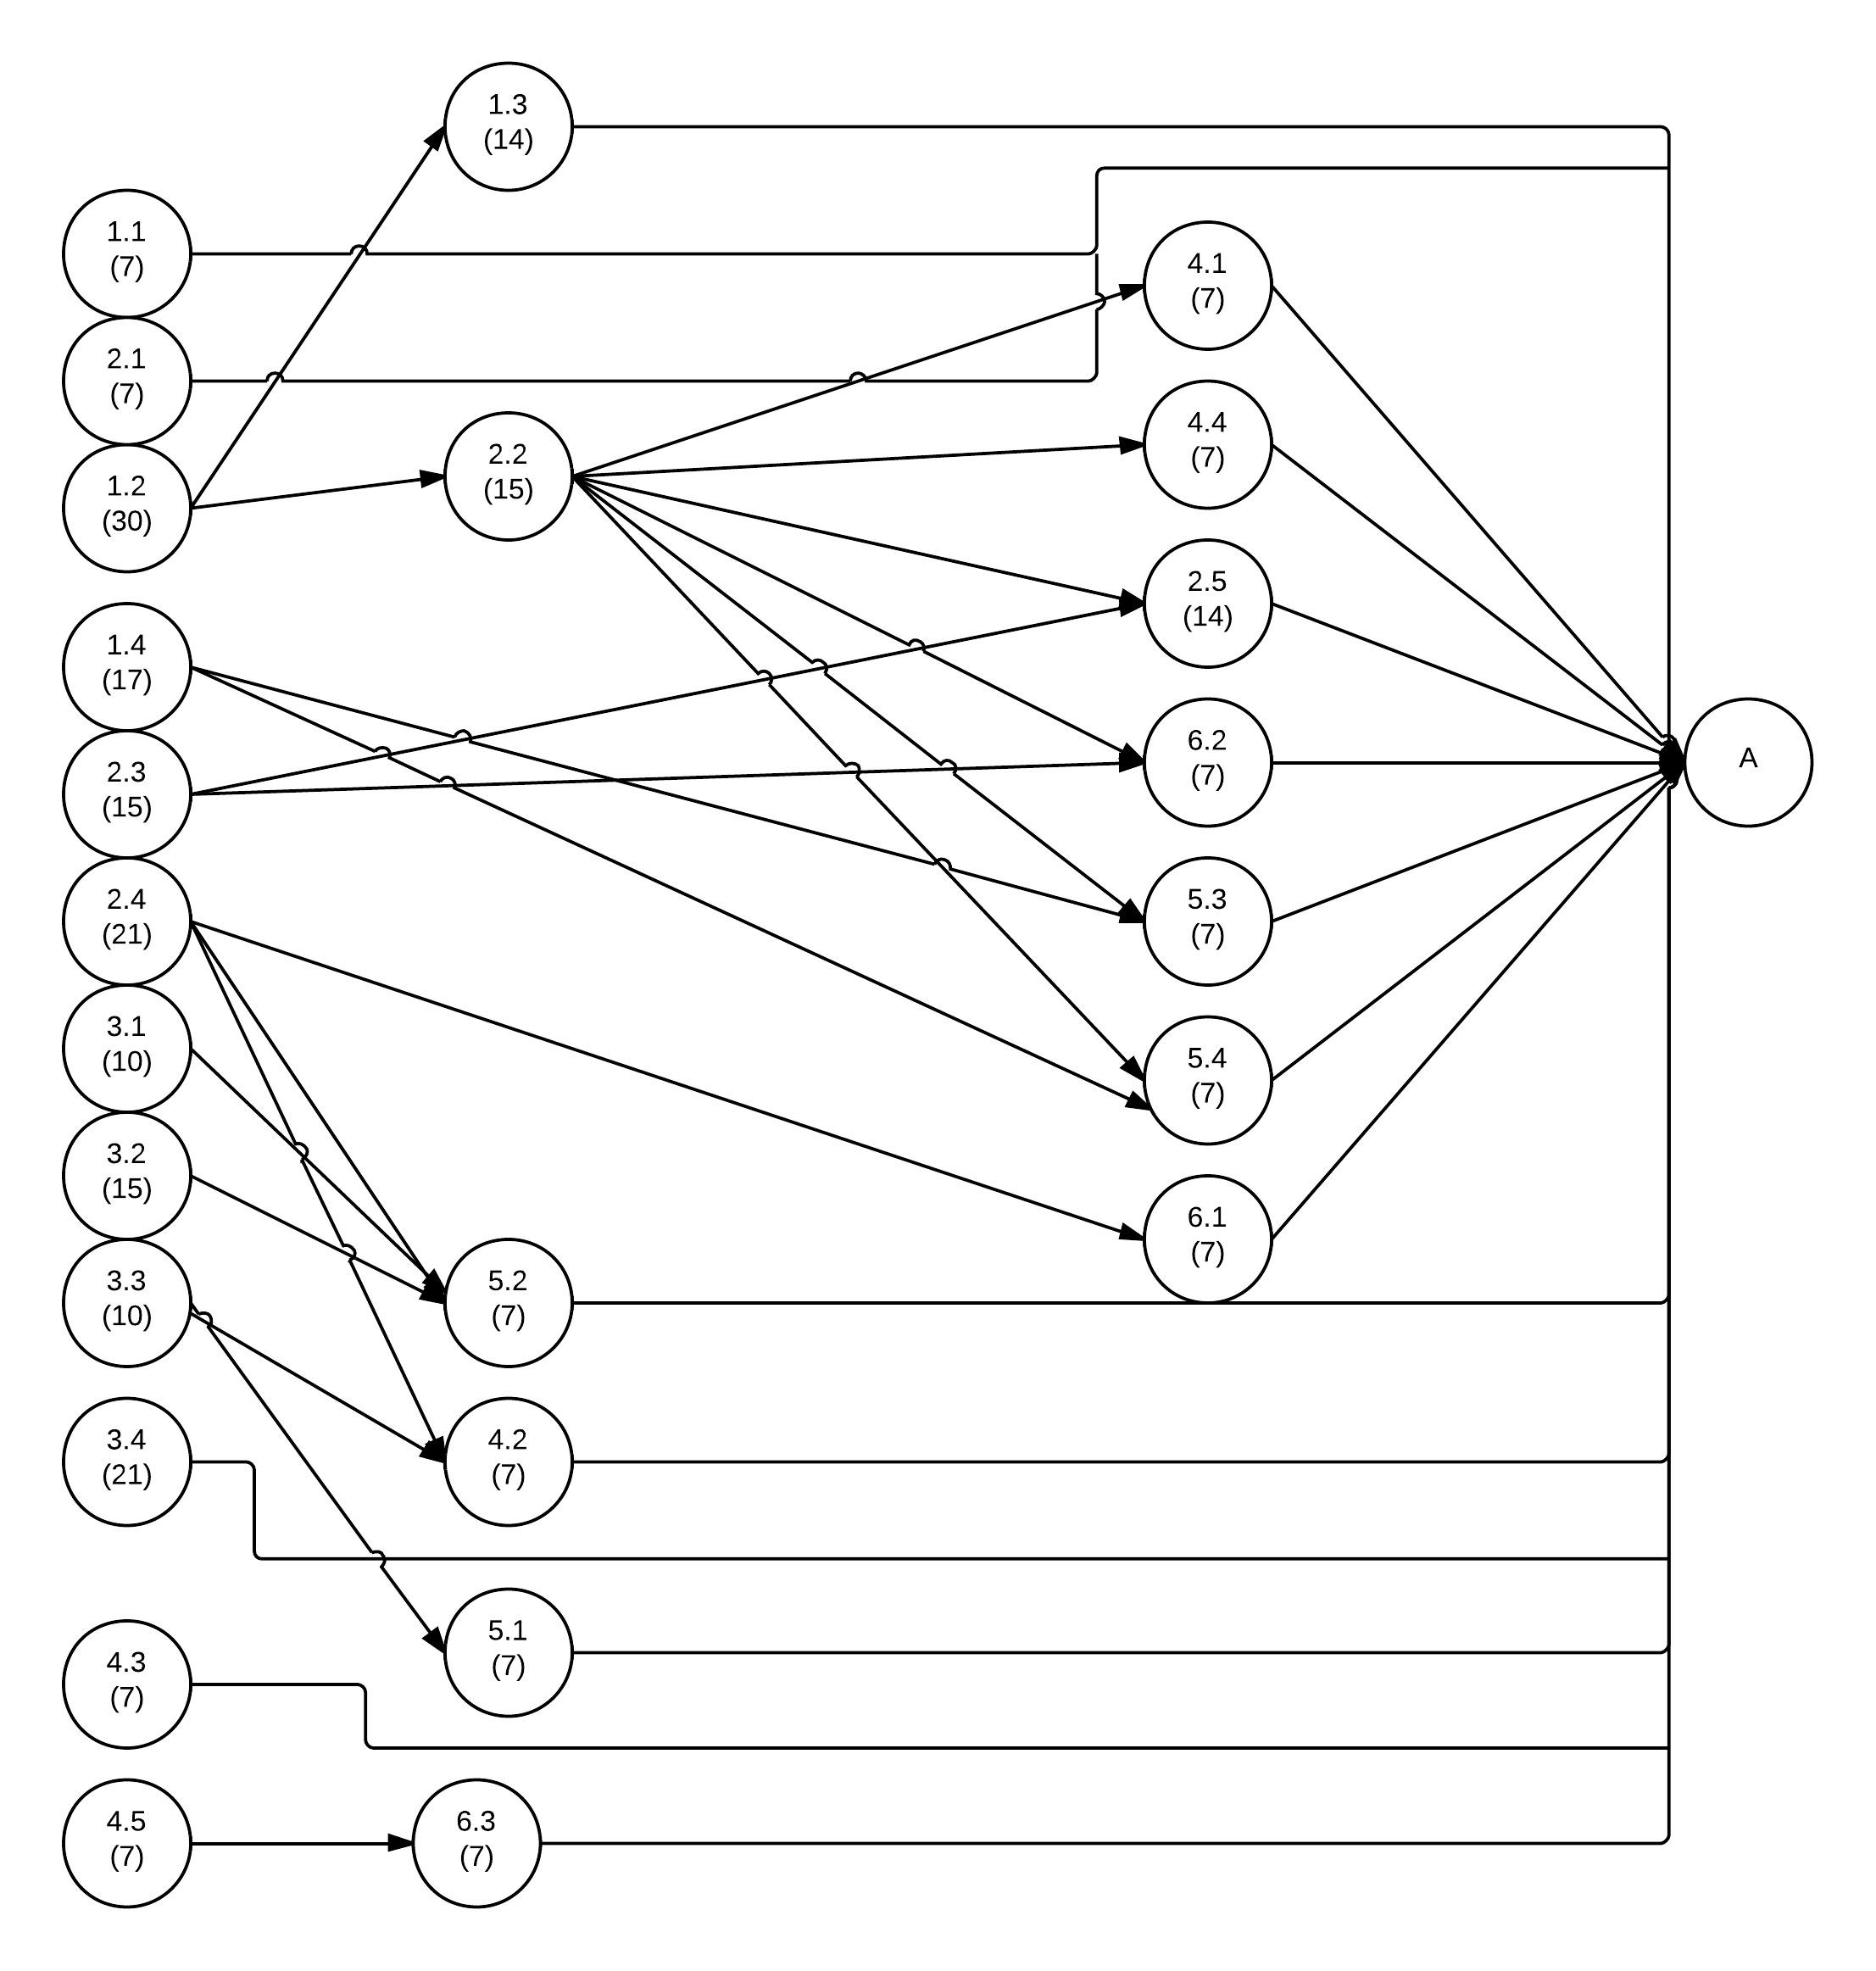
\includegraphics[width=1\textwidth]{AON.jpeg}
\caption{Activity on Node}
\label{fig:Activity on Node}
\end{figure}
\section{Gantt Chart Schedule}
\begin{figure}[H]
\centering
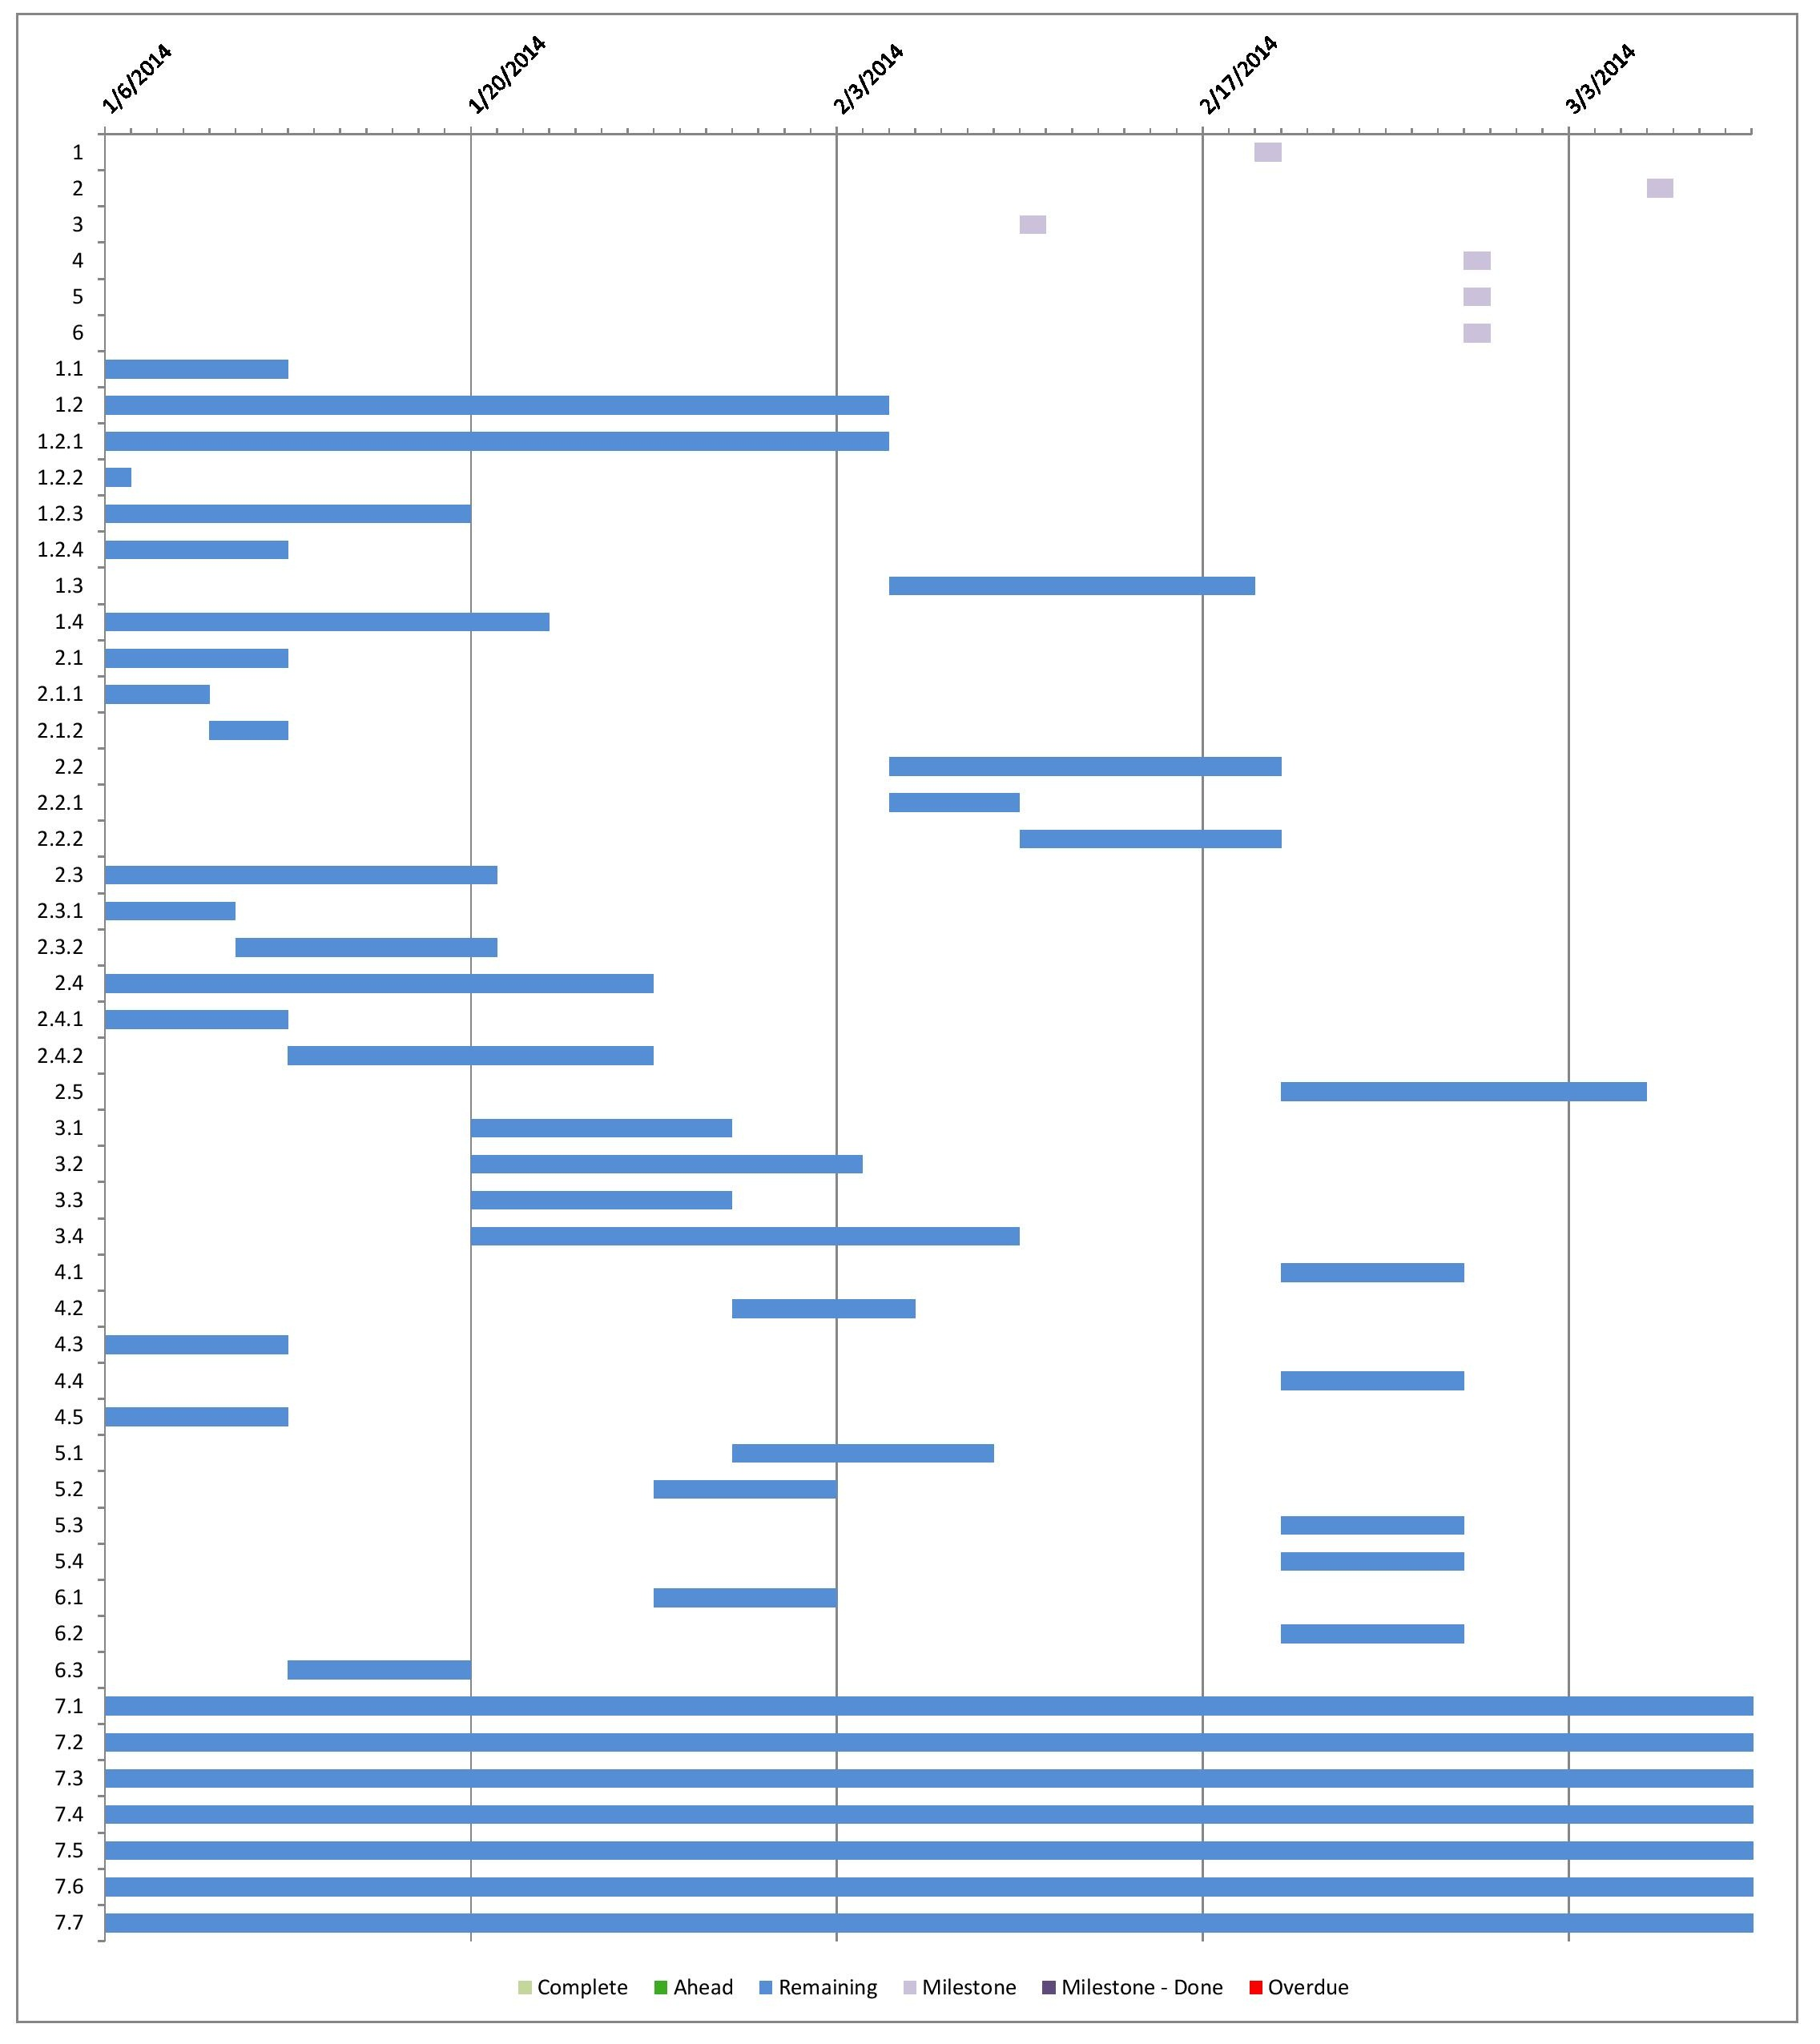
\includegraphics[width=1\textwidth]{gantt.jpg}
\caption{Gantt Chart}
\label{fig:Gantt Chart}
\end{figure}
\subsection{Landmark Schedule}
Each landmark is marked on the Gantt Chart with a purple square.
\subsection{Critical Design Review Schedule}
Critical design reviews will happen every two weeks, marked on the Gantt Chart by the vertical lines.
Critical design review will end after 6 weeks. By this point the critical parts of the project should be finalized. 
\subsection{\gls{wbs} and \gls{lrc} Review and Update Schedule}
Chart updates will happen every two weeks, denoted by both the solid and dashed vertical red lines.
\section{Budget}
\begin{longtable}{|>{\centering}m{3.0cm}|>{\centering}m{1.8cm}|>{\centering}m{1.8cm}|>{\centering}m{1.8cm}|>{\centering}m{1.8cm}|>{\centering}m{2.3cm}|m{1.8cm}|}
	\caption{Budget}
	\label{table:primary} \\
	\hline \textbf{Item} & \textbf{Required} & \textbf{Purchase} & \textbf{Cost} & \textbf{Total} & \textbf{Specification} &\textbf{Supplier}\\ \hline
	\endfirsthead
	\multicolumn{7}{c}{\tablename\ \thetable\ -- \textit{Continued from previous page}} \\ \hline
	 \textbf{Item} & \textbf{Required} & \textbf{Purchase} & \textbf{Cost} & \textbf{Total} & \textbf{Specification} &\textbf{Supplier}
	\endhead 
	\multicolumn{7}{r}{\textit{Continued on next page}} \\
	\endfoot \hline
	\endlastfoot

	Motor Driver Unit&4 &5& \$14.95& \$74.75&DRV 8825&Pololu\\ \hline
	Motor Controller Development Board&1&2&\$35.00&\$70.00& RasPi 512MB&Newark\\ \hline
	Master Controller Development Board&1&2&\$35.00&\$70.00&MSP430 FR5739 Dev Kit&TI\\ \hline
	Peripheral Components&1&2&\$30.00&\$60.00&Misc on-board electronics&Tayda\\ \hline
	Motor Connection Hardware&4&5&\$10.00&\$50.00&8 Pin Mil-Spec Connectors&eBay\\ \hline
	Power Supply Unit&1&2&\$25.00&\$50.00&10A, Switching PSU&eBay\\ \hline
	Testing Materials&1&1&\$50.00&\$50.00&Stuff to carve up&Lowes\\ \hline
	Enclosure&1&1&\$50.00&\$50.00&Fabricate in house&Lowes\\ \hline
	Monitor for\\Master Controller&1&1&\$35.00&\$35.00&HDMI compatible (used)&GoodBytes\\ \hline
	Cabling \& Test Harness&1&2&\$10.00&\$20.00&Wire is expensive&eBay\\ \hline
	Voltage Regulation&2&3&\$6.00&\$18.00&DC-DC Converter&eBay\\ \hline
	Total &&&&\$547.75&&\\ \hline
\end{longtable}
\section{Engineering Hours}

\begin{table}[H] 
\caption{Engineering Hours}
	\label{table:engineeringhours}
	\centering 
\begin{tabular}{|r|c|}
	
	\hline Josh DeWitt&150\\ \hline
	James Gehringer&150\\ \hline
	Evan Milton&150\\ \hline
	Chad Staley&150\\ \hline
	Total&600\\ \hline
\end{tabular}
\end{table} 
